
{\fontfamily{phv}\selectfont
\enlargethispage{2cm}

\hspace*{25mm}
\parbox{14cm}{%
{\huge \textbf{Math Test -- No Calculator}}\\

{\Large \textbf{25 MINUTES, 20 QUESTIONS}} \\[3mm]


\textbf{Turn to Section 3 of your answer sheet to answer the questions in this section.}\\[2mm]
%
}
\hrule height 1pt

\vspace*{5mm}

%%%%%%%%%%%%%%%%%%%%%%%%%%%%%%%%%%%%%%%%%
% Directions
%%%%%%%%%%%%%%%%%%%%%%%%%%%%%%%%%%%%%%%%%

\hspace*{25mm}
\parbox{14cm}{%
\raggedright
\colorbox{black}{\color{white}\textbf{\small DIRECTIONS}}\hskip-2pt

\vspace*{5mm}

\textbf{For questions 1-15}, solve each problem, choose the best answer from the choices\\
provided, and fill in the corresponding circle on your answer sheet. \textbf{For questions 16-20},\\
solve the problem and enter your answer in the grid on the answer sheet. Please refer to\\
the directions before question 16 on how to enter your answers in the grid. You may use\\
any available space in your test booklet for scratch work.
}

\vspace*{3mm}

%%%%%%%%%%%%%%%%%%%%%%%%%%%%%%%%%%%%%%%%%
% Notes
%%%%%%%%%%%%%%%%%%%%%%%%%%%%%%%%%%%%%%%%%

\hspace*{25mm}
\parbox{15cm}{%
\raggedright
\colorbox{black}{\color{white}\textbf{\small NOTES}}\hskip-2pt

\vspace*{0mm}

\begin{enumerate}[itemsep=0mm,leftmargin=5mm]
	\item The use of a calculator \textbf{is not permitted}.
	\item All variables and expressions used represent real numbers unless otherwise indicated.
	\item Figures provided in this test are drawn to scale unless otherwise indicated.
	\item All figures lie in a plane unless otherwise indicated.
	\item Unless otherwise indicated, the domain of a given function f is the set of all real numbers x for which f(x) is a real number.
\end{enumerate}	
	}

\vspace*{0mm}


%%%%%%%%%%%%%%%%%%%%%%%%%%%%%%%%%%%%%%%%%
% Reference
%%%%%%%%%%%%%%%%%%%%%%%%%%%%%%%%%%%%%%%%%

\hspace*{25mm}
\parbox{15cm}{%
\raggedright
\colorbox{black}{\color{white}\textbf{\small REFERENCE}}\hskip-2pt

\vspace*{4mm}

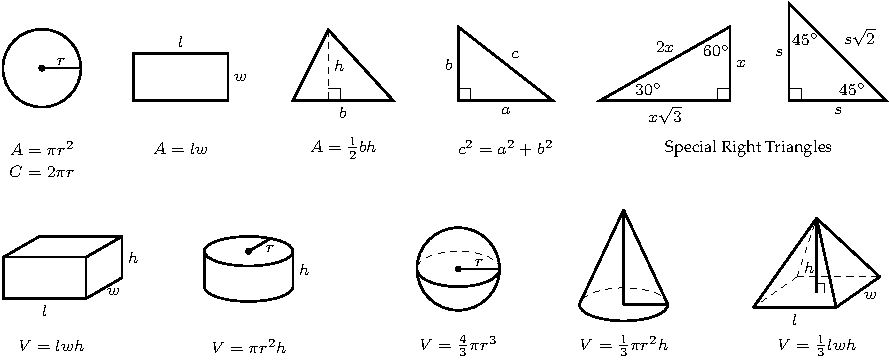
\includegraphics{support/sat_2016_math_formula_key.pdf}

\vspace*{2mm}

The number of degrees of arc in a circle is 360.\\[1ex]

The number of radians of arc in a circle is 2$\pi$.\\[1ex]

The sum of measures in degrees of the angles of a triangle is 180.}

\vspace*{4mm}

\hrule height 1pt
}

\clearpage

